\newpage
\section{Auswertung}

In diesem Abschnitt wird der Versuc hausgewertet.

\subsection{gedämpften Schwingung}
Zunächst wird bei einer gedämpften Schwingung die Zeitabhängigkeit der Amplitude untersucht, um den effektiven Dämpfungswiderstand bestimmen zu können.
Dabei wird zunächst die in der Messung bestimmte Amplitudenspitzen in die \autoref{tab:1} eingetragen.

\begin{table}
    \centering
    \caption{Gemessene Spannungsamplituden in Abhängigkeit von der Zeit}
    \label{tab:1}
    \begin{tabular} {S[table-format=4.1] S[table-format=2.2]}
        \toprule
        {$t \mathbin{/} \si{\micro\second}$} & {$U \mathbin{/} \si{\volt}$}  \\
    \midrule
    0 	    & \,\,  -82   \\
    12.5 	& \,\,   76   \\
    25.5	& \,\,  -64   \\
    40  	& \,\,   56   \\
    55	    & \,\,  -48   \\
    67.5	& \,\,   40   \\	
    80	    & \,\,  -36   \\
    93.75	& \,\,   32   \\
    107.5	& \,\,  -26   \\
    122.5	& \,\,   22   \\
    135	    & \,\,  -20   \\
    148.75  & \,\,	 16   \\
    162.5	& \,\,  -14   \\
    175	    & \,\,   11   \\
    188.75  & \,\,	-10   \\
    202.5	& \,\,   9    \\
    216.25  & \,\,	-8    \\
    \bottomrule
\end{tabular}
\end{table}

\noindent
Es reicht jedoch die Einhüllende zu betrachten. Da die Einhüllende unterhalb der X-Achse und Oberhalb sich um einen Vorzeichen unterscheiden, kann 
zur Modelierung dieser, lediglich der Betrag der gemessen Spannung betrachtet werden. Daraus folgen die Grafiken (\ref{fig:1}), in welcher die Zeit gegen die Spannung und gegen den 
Spannungsbetrag aufgetragen werden.

\newpage
\begin{figure}
    \centering
    \label{fig:1}
    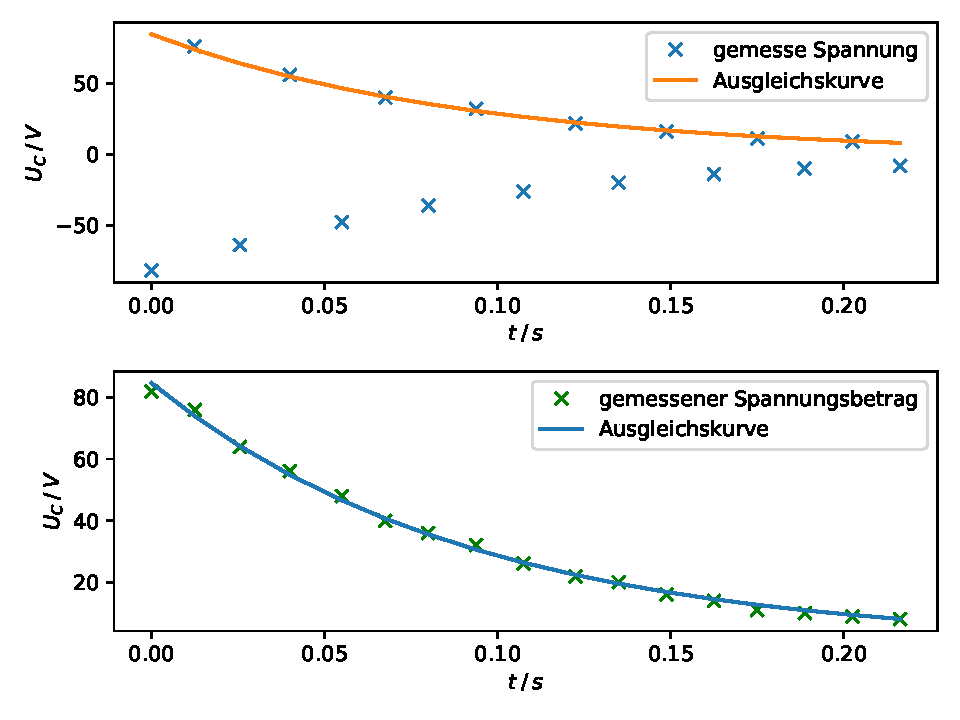
\includegraphics{Daten/a.pdf}
    \caption{Gemessene Spannungsamplituden mit Ausgleichsfunktion}
\end{figure}

Um die Einhüllende zu modelieren, kann diese in der Form
\begin{equation}
    U = a \symup{e}^{b*t}
\end{equation}

\noindent
angenommen werden. Aus der Theorie gilt mit der \autoref{eqn:einh} der Zusammenhang $a = U_0$ und $b = -2 \pi \mu$. Daraus folgt %U_0 e^-2*pi*my*t


\begin{align*}
    a &= 0.0846 \pm 0.0008 \Leftrightarrow U_0 = 0.0846 \pm 0.0008 \si{\volt} \\
    b &= -10852.9624 \pm 174.9926 \Leftrightarrow \mu = 1727.3026 \pm 27.8509 \si{\per\second} \, .\\
\end{align*}

\noindent
Mit der Beziehung 
\begin{equation}
    R_\text{eff} = 4\pi\mu L = -2 L b
\end{equation}

\noindent
lässt sich der Dämpfungswiderstand R, mit $L = 3.5 \pm 0.01 \si{\milli\henry}$ zu
\begin{equation*}
    R_\text{eff} = 76 \pm 1,2 \si{\ohm}
\end{equation*}
<<<<<<< HEAD

\noindent
bestimmen. Damit ist die Abweichung des verbauten Widerstands $R = 30,3 \pm 0,1 \si{\ohm}$ $151 \pm 0.04 \si{\percent}$.
||||||| c59dd00
bestimmen. Damit ist die Abweichung des im verbauten Widerstands $R = 30,3 \pm 0,1 \si{\ohm}$ $99.749 \pm 00.004 \si{\percent}$.
=======
bestimmen. Damit ist die Abweichung des verbauten Widerstands $R = 30,3 \pm 0,1 \si{\ohm}$ $99.749 \pm 00.004 \si{\percent}$.
>>>>>>> d61d3707ca741e5717fac4d4393cf9724ddb3269

\noindent
Die Abklingdauer kann mithilfe der Formel 
\begin{equation*}
    T_\text{ex} = \frac{1}{2\pi\mu} = - \frac{1}{b}
\end{equation*}
berechnet werden zu
\begin{align*}
    T_\text{ex} = 92,1 \pm 1,5 \si{\micro\second} \, . \\
\end{align*}



\subsection{aperiodische Grenzfall}
Zusätzlich lässt sich der Dämpfungswiderstand $R_\text(ap)$ experimentell bestimmen zu $R_ap = 12,725 \si{\ohm}$. Der theoretische Wert lässt sich mit der Formel (\ref{eqn:rap}) %R = 2(L/C)^1/2
mit den gegeben Werten
\begin{align*}
   R &= 30,3 \pm 0,1 \, \si{\ohm} \\
   L &= 3,5 \pm 0,01 \, \si{\milli\henry} \\
   C &= 5 \pm 0 \, \si{\nano\farad} \\
\end{align*}

\noindent
aus dem Aufbau bestimmen. Daraus folgt das $$ R_\text{ap} = 1673.3 \pm 2.4 \, \si{\ohm} $$ und eine Abweichung von $ 660.46 \, \si{\percent}$.

\subsection{Frequenzabhängigkeit der Kondensatorspannung}

Die gemessene Kondensatorspannung $U_C$ und die dazugehörige Frequenz $\omega$ wird in die \autoref{tab:2} eingetragen und 
der Quotient $\frac{U_C}{U_\text{Err}}$ gegen die Frequenz $\omega$ halblogarithmisch in die \autoref{fig:2} aufgetragen.

\begin{table}
    \centering
    \caption{Messwerte zur Kondensator- und Erregerspannung}
    \label{tab:frequence}
    \begin{tabular} {S[table-format=2.2] S[table-format=1.2] S[table-format=1.2] S[table-format=1.2]}
        \toprule
        {$\nu \mathbin{/} \si{\kilo\hertz}$}&
        {$U_\text{C} \mathbin{/} \si{\volt}$} & {$U_\text{Err} \mathbin{/} \si{\volt}$}   \\
        \midrule
        10		    &        50			&         50
        15		    &        55			&         50
        20		    &        65			&         50
        25		    &        87.5		&         50
        30		    &        130		&	      50
        32		    &        177.5		&         50
        34		    &        265		&	      40
        36		    &        430		&	      30
        38		    &        405		&	      30
        40		    &        235		&	      40
        42		    &        150		&	      50
        45		    &        97.5		&         50
        50		    &        55			&         50
        55		    &        40			&         50
        58		    &        32			&         50		
        \bottomrule
    \end{tabular}
\end{table}

\begin{figure}
    \centering
    \label{fig:1}
    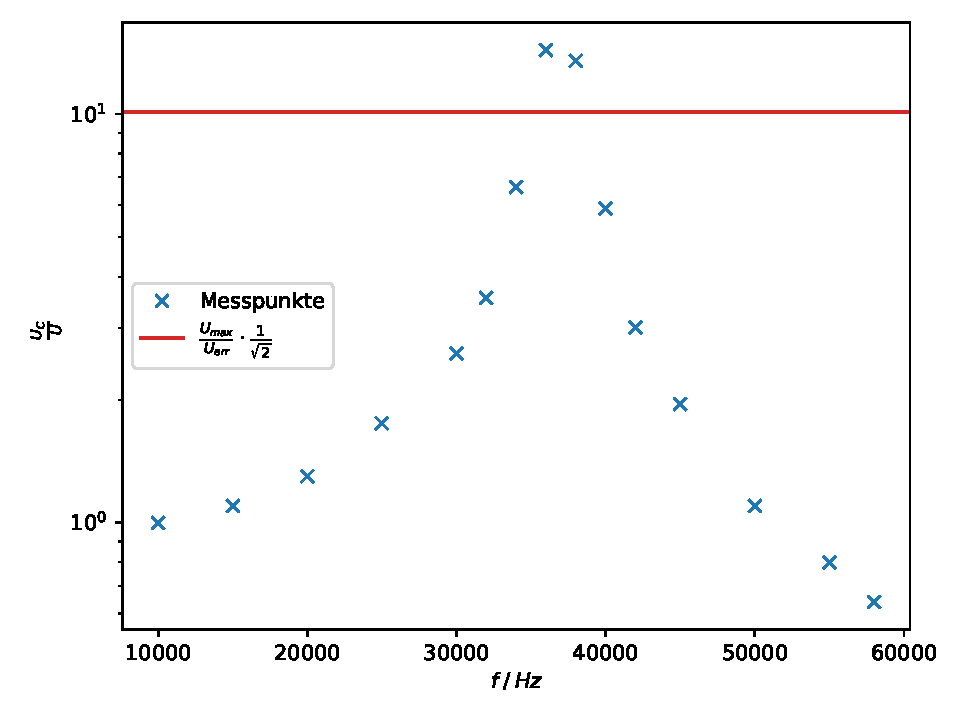
\includegraphics{Daten/c.pdf}
    \caption{Quotient $\frac{U_C}{U_\text{Err}}$ gegen die Frequenz $\omega$ halblogarithmisch aufgetragen}
\end{figure}


\noindent
Aus der Grafik lässt sich für die Frequenzen, bei denen die Spannung den Wert $\frac{U_\text{max}}{U_\text{Err}}\frac{1}{\sqrt{2}}$ erreicht, entnehmen als

\begin{align*}
    \omega_+ &= \SI{35,1} \pm 0,3 \,  {\kilo\hertz} \\
    \omega_- &= \SI{38,5} \pm 0,3 \,  {\kilo\hertz} \, .
\end{align*}

\noindent
Daraus folgt die Breite 
\begin{equation*}
    b = 3,4 \pm 0,3 \si{\kilo\hertz} \, .
\end{equation*}

Für die Güte kann mit der \autoref{eqn:guete} $$ q = 70 \pm 6 \, $$ berechnet werden. 

\noindent
Die theoretische Breite der Ressonanzkurve lässt sich der \autoref{eqn:wmp} nähern. Mithilfe dieser Näherung lässt sich die Breite der Ressonanzkurve und die Güte berechnen zu %w+ - w- = R/L

\begin{align*}
    b & = 8.657 \pm 0.025 \si{\kilo\hertz}\\
    q & = 27.61\pm 0.04 \, . 
\end{align*}




